\Gls{ml} is the application of statistics, algorithms and computing power to discover meaning and/or devise actions from data.
\gls{ml} has become an umbrella term, encompassing the family of algorithms
    which aim to leverage computers to learn without being explicitly programmed,
    as opposed to the more general \gls{ai}, which seeks to make computers behave intelligently,
    admitting explicit programs to achieve tasks \cite{MLvAI}.
Its history is therefore imprecise since a number of early, apparently unrelated algorithms were proposed independently, 
    which now constitute \gls{ml} routines \cite{mcculloch1943logical, turing2009computing}. 
Nevertheless, the field of \gls{ml} has been advancing rapidly since the second half of the $20^{\textrm{th}}$ century \cite{russell2002artificial}, 
    especially recently due to the availability of advanced hardware such as \glspl{gpu}, 
    facilitating significant progress through an ever-increasing aresnal of powerful open source software \cite{pedregosa2011scikit, abadi2016tensorflow, paszke2019pytorch}. 
\par 

Throughout this thesis, we endeavour to combine known methods from the \gls{ml} literature with capabilities of \glspl{qc}\footnotemark. 
Typical \gls{ml} algorithms, which rely on \glspl{cpu} or \glspl{gpu}, are deemed \emph{classical} \glsentrylong{ml},
    in contrast with \gls{qml}, where \glspl{qc} are central to processing the data.
Similarly to the remit of \cref{chapter:qm}, here we do not provide an exhaustive account of \gls{ml} algorithms:
    rather, we describe only the algorithms which are used in later chapters, 
    referring readers to standard texts for a wider discussion \cite{russell2002artificial, hastie2009elements}.

\footnotetext{Or simulated \glspl{qc}, in this thesis.}


\section{Classical \glsentrylong{ml}}\label{sec:classical_ml}

Of course the first step in any \gls{ml} application is to consider the types of available data,
    with respect to the ensemble of known algorithms. 
Classical \gls{ml} is usually described in three categories,
    broadly based on the format of data on which the insight can be built;
    we will briefly describe each to provide context to discussions throughout this thesis. 
Later in this thesis we will use the word \emph{model} for descriptions of quantum systems, 
    but here \emph{model} refers to the mapping between inputs and outputs which the \gls{ml} algorithm devises.
\par 

\subsection{Supervised \glsentrylong{ml}}
Models are trained using \emph{labelled} data, 
    i.e. each training sample has a known label $y_i$;
    or, a set of \emph{feature vectors} $\left\{\vec{x}_i\right\}$ are associated with the set of 
    corresponding \emph{classes} $\left\{ y_i \right\}$ \cite{caruana2006empirical}. 
The output is a predictive tool which aims to reconstruct the classes of unseen feature vectors:
    in general, we can view the role of \gls{ml} in this setting as distilling the function $f$ such that 
\begin{equation}
    \label{eqn:supervised_ml_target}
    f : \vec{x}_i \longmapsto y_i \ \ \ \  \forall (\vec{x}_i, y_i).
\end{equation}
\par 

\par 

For an incomplete list of common supervised algorithms, 
    we list examples in \cref{table:supervised_examples},
    with definitions:
\begin{easylist}
    & \emph{Classification}: models which can assign unseen instances the most appropriate 
        label from a fixed set of available labels  \cite{kotsiantis2007supervised};
    & \emph{Linear regression}: models capture the linear relationship between numerical features and the target scalar, 
        by determining linear coefficients for each feature. 
    & \emph{Neural networks}\footnote{including {deep learning} networks}: \emph{universal function approximators}.
        By invoking a set of linear and non-linear transformations on input data, 
        where the network is a function of some paramterisation $w$, 
        finding the optimal network such that \cref{eqn:supervised_ml_target} is satisfied, 
        $f(\vec{x}_i | w) = y_i$. 
\end{easylist}
\par 

\begin{table}
    \begin{center}
    \begin{tabular}{llcc}
        Algorithm & Output $y$ & Input $\vec{x}$ \\
        \hline
        Classification & Category: animal & $ \left( \textrm{height, weight, # legs}\right) $ \\
        Linear regression & Number: salary & $\left( \textrm{age, seniority, years\_experience}\right) $ \\
        Neural network & Number: salary & $\left( \textrm{age, seniority, years\_experience}\right) $ \\
        Support Vector Machine & & \\ 
    \end{tabular}
    \end{center}
    \caption[Supervsied learning algorithm examples]{Supervsied learning algorithm examples}
    \label{table:supervised_examples}
\end{table}

Supervised \gls{ml} rely on the existence of a body of labelled samples -- the dataset $\mathcal{D}$ -- upon which the model can be trained.
An important aspect of these algorithms is assessment, i.e. judging their performance. 
By definition of the data format, this is a straightforward task for supervised routines:
    the classes assigned to feature vectors can be quantitatively assessed. 
The task of the machine is then to learn the configuration, $w$, for which this is satisifed in the highest proportion of cases. 


\subsection{Unsupervised \glsentrylong{ml}}

An example of supervised \gls{ml} is

\subsection{\Glsentrylong{rl}}

An example of \gls{rl} is self driving cars. 
Agency...

\section{Quantum \glsentrylong{ml}}
\begin{easylist}[itemize]
    & distinctions
    && q data q hardware $\rightarrow$ pure QML
    && q data classical hardware $\rightarrow$ ml for q physics
    && classical data q hardware $\rightarrow$ q enhanced ml
    && classical data c hardware $\rightarrow$ wrong thesis (\cref{sec:classical_ml})

    & examples/applications of QML 
    && QNN, q svm, 
    & Remit of this thesis $\rightarrow$ ml for q physics
    && i.e. using data from quantum system and/or hardware but in conjunction with classical co-processor, 
        for the study of quantum systems
\end{easylist}
\cite{dunjko2018machine}

\section{\glsentrylongpl{ga}}\label{sec:genetic_algorithms}
In later chapters we will use a class of optimisation techniques known as \emph{evolutionary algorithms} \cite{back1996evolutionary, de2020evolutionary}.
In particular, \emph{\glsentryfullpl{ga}} are central to our primary applications, 
    specifically in \cref{chapter:ga}.
Here we describe \glspl{ga} in general terms for reference in later chapters. 
\par 
\glspl{ga} work by assuming a given problem can be optimised, if not solved, by a single candidate 
    among a fixed, closed space of candidates, called the population, $\population$. 
A number of candidates are sampled at random from $\population$ into a single \emph{generation}, 
    and evaluated through some \glsentryfull{of}, which assesses the fitness of the candidates at solving the problem of interest. 
Candidates from the generation are then mixed together to produce the next generation's candidates: 
    this \emph{crossover} process aims to combine only relatively strong candidates, such that the average 
    candidates' fitness improve at each successive generation, 
    mimicing the biological mechanism whereby the genetic makeup of offspring is an even mixture of both parents
    through the philosophy of \emph{survival of the fittest}. 
The selection of strong candidates as parents for future generations is therefore imperative; 
    in general parents are chosen according to their fitness as determined by the \gls{of}. 
Buidling on this biological motivation, much of the power of \glspl{ga} comes from the concept of \emph{mutation}: 
    while offspring retain most of the genetic expressions of their parents, some elements are mutated at random.
Mutation is crucial in avoiding local optima of the \gls{of} landscape
    by maintaining diversity in the examined subspace of the population.
\par 

Pseudocode for a generic \gls{ga} is given in \cref{alg:ga},
    but we can also informally define the procedure as follows. 
Given access to the population, $\population$, 

\begin{easylist}[enumerate]
    \ListProperties(Numbers2=l, Numbers3=r)
    & Sample $N_m$ candidates from the population at random
    && call this group of candidates the first generation, $\mu$. 
    & \label{ga:loop} Evaluate each candidate $\gamma_j \in \mu$
    && each $\gamma_j$ is assigned a fitness, $g_j$;
    && the fitness is computed through an objective function acting on the candidate, i.e. $g_j = g(\gamma_j)$. 
    & Map the fitnesses of each candidate, $\{g_j\}$, to selection probabilities for each candidate, $\{s_j\}$
    && e.g. by normalising the fitnesses, or by removing some poorly-performing candidates and then normalising. 
    & Generate the next generation of candidates
    && Reset $\mu = \{ \}$;
    && \label{ga:select} Select pairs of parents, $\left\{\gamma_{p_1}, \gamma_{p_2}\right\}$, from $\mu$
    &&& Each candidate's probability of being chosen is given by their $s_j$.
    && Cross over $\left\{\gamma_{p_1}, \gamma_{p_2}\right\}$ to produce children candidates, $\left\{\gamma_{c_1}, \gamma_{c_2}\right\}$
    &&& mutate $\gamma_{c_1}, \gamma_{c_2}$ according to some random probabilistic process;
    &&& keep $\gamma_{c_i}$ only if it is not already in $\mu$, to ensure $N_m$ unique candidates are tested at each generation.
    && until $|\mu| = N_m$, iterate to step (\ref{ga:select}.
    & Until the $N_g^{th}$ generation is reached, iterate to step \ref{ga:loop};
    & The strongest candidate on the final generation is deemed the solution to the posed problem. 
\end{easylist}


\begin{algorithm}
    \caption{Genetic algorithm}
    \label{alg:ga}
    \DontPrintSemicolon
    \KwIn{ $\population$ \tcp*[1]{Population of candidate models}}
    \KwIn{ $g()$ \tcp*[1]{objective funtion}}
    \KwIn{ $\ttt{map\_g\_to\_s}()$ \tcp*[1]{function to map fitness to selection probability}}
    \KwIn{ $\ttt{select\_parents}()$ \tcp*[1]{function to select parents among generation}}
    \KwIn{ $\ttt{crossover}()$ \tcp*[1]{function to cross over two parents to produce offspring}}
    \KwIn{ $N_g$ \tcp*[1]{number of generations}}
    \KwIn{ $N_m$ \tcp*[1]{number of candidates per generation}}\;

    \KwOut{$\gamma^{\prime}$ \tcp*[1]{strongest candidate}}\;
    
    $\mu \gets \ttt{sample} \left( \population, N_m\right)$\; 

    \For{$i \in 1, ..., N_g$}{
        \For{$\gamma_j \in \mu$ }{
            $g_j \gets g(\gamma_j) $ \tcp*[1]{assess fitness of candidate}
        }

        $\{ s_j \}  \gets \ttt{ map\_g\_to\_s}(\{g_j \})$ \tcp*[1]{map fitnesses to normalised selection probability}
        $\mu_c = \argmax\limits_{s_j} \{ \gamma_j \}$ \tcp*[1]{record champion of this generation}\;

        $\mu \gets \{ \}$ \tcp*[1]{empty set for next generation}

        \While{$| \mu | < N_m$}{
            $p_1, p_2 \gets \ttt{select\_parents}(\{s_j\})$ \tcp*[1]{choose parents based on candidates' $s_j$}
            $c_1, c_2 \gets \ttt{crossover}(p_1,p_2)$ \tcp*[1]{generate offspring candidates based on parents}

            \For{$c \in \{c_1, c_2\}$ }{
                \If{$c \notin \mu$}{
                    $\mu \gets \mu \cup \{ c\}$ \tcp*[1]{keep if child is new} 
                }
            }
        }
    }

    $\gamma^{\prime} \gets \argmax\limits_{s_j}\{ \gamma_j \in \mu \}$ \tcp*[1]{strongest candidate on final generation}\;

    return $\gamma^{\prime}$

\end{algorithm}


\par 

Candidates are manifested as \emph{\glspl{chromosome}}, i.e. strings of fixed length, 
    whose entries, called  \emph{\glspl{gene}}, each represent some element of the system.
In general, \glspl{gene} can have continuous values, although usually, and for all purposes in this thesis, 
    genes are binary, capturing simply whether or not the \gls{gene}'s corresponding feature is present 
    in the \gls{chromosome}. 

\subsection{Example: knapsack problem}\label{sec:knapsack}
\begin{figure}
    \begin{center}
        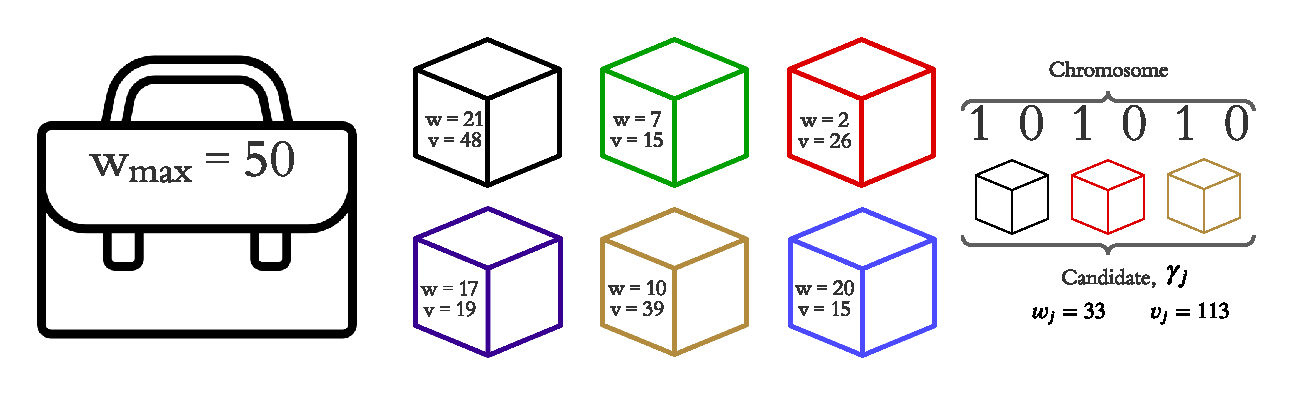
\includegraphics[width=\textwidth]{theoretical_study/figures/knapsack_schematic.pdf}
    \end{center}
    \caption[Knapsack problem]{
        Depiction of the knapsack problem.
        \textbf{Left}, A knapsack which can hold any number of objects but is constrained by the total weight it can support, 
        $w_{max} = 50$. 
        \textbf{Centre}, A set of objects are available, each with associated weight, $w$, and value $v$. 
        The objective is to find the subset of objects which maximise the total value, 
        while not exceeding the capacity of the knapsack. 
        \textbf{Right}, An example chromosome, i.e. candidate $\gamma_j$, where the bits of the chromosome indicate 
            whether the corresponding object is included, allowing for calculation of the total weight and value of 
            the candidate, $w_{j}, v_{j}$. 
    }

\end{figure}
One commonly referenced combinatorial optimisation problem is the \emph{knacksack problem}: 
    given a set of objects, where each object has a defined mass and also a defined value, 
    determine the set of objects to pack in a knapsack which can support a limited weight, 
    such that the value of the packed objects is maximised. 
Say there are $n$ objects, 
    we can write the vector containing the values of those objects as $\vec{v}$, 
    and the vector of their weights as $\vec{w}$. 
We can then represent configurations of object sets as candidate vectors $\vec{\gamma}_j$, 
    whose genes are binary, and simply indicate whether or not the associated object is included in the set. 
For example, with $n=6$,
\begin{equation}
    \gamma_j = \ttt{100001} \Longrightarrow \vec{\gamma}_j = \irow{1 & 0 & 0 & 0 & 0 & 1},
\end{equation} 
indicates a set of objects consisting only of those indexed first and last, with none of the intermediate objects included. 

\par
The fitness of any candidate is then given by the total value of that configuration of objects, $v_j = \vec{v} \cdot \vec{\gamma}_j$, 
    but candidates are only admitted\footnotemark \ if the weight of the corresponding set of objects 
    is less than the capacity of the knapsack, i.e. $\vec{w}_j \cdot \vec{\gamma}_j \leq w_{max}$. 
\footnotetext{
    Note there are alternative strategies to dealing with candidates who violate the weight condition, 
    such as to impose a penalty within the \gls{of}, but for our purposes let us assume we simply disregard violators. 
}
\par 

For example where each individual object has value $<50$ and weight $<25$ and $w_{max} = 50$, 
recalling $\gamma_j = \ttt{100001}$, say, 
\begin{subequations}
    \begin{equation}
        \vec{ v } = \irow{ 48 & 15 & 26 & 19 & 39 & 15 } \Longrightarrow v_j = \vec{\gamma}_j \cdot \vec{v} = 48 + 15 = 63;
    \end{equation}
    \begin{equation}
        \vec{ w } = \irow{ 21 & 7 & 2 & 17 & 10 & 20 } \Longrightarrow w_j = \vec{\gamma}_j \cdot \vec{w} = 21 + 20 = 41.
    \end{equation}
\end{subequations}
We can hence assess the fitness of $\gamma_j$ as $63$ and deem it a valid candidate since it does not exceed the weight threshold.
We can likewise compute the total weight and value of a series of randomly generated candidates, 
    and deem them valid or not. 
\cref{table:knapsack_candidates} shows a set of 12 randomly generated candidates, 
    of which ten are valid.

\begin{table}[H]
    \begin{center}
        \begin{tabular}{lrrl}
\hline
{} &                                    Value &                                   Weight &                                    Valid \\
Candidate                                &                                          &                                          &                                          \\
\midrule
110000                                   &                                       63 &                                       28 &                                      Yes \\
000011                                   &                                       54 &                                       30 &                                      Yes \\
011101                                   &                                       75 &                                       46 &                                      Yes \\
101010                                   &                                      113 &                                       33 &                                      Yes \\
000101                                   &                                       34 &                                       37 &                                      Yes \\
010111                                   &                                       88 &                                       54 &                                       No \\
011011                                   &                                       95 &                                       39 &                                      Yes \\
110011                                   &                                      117 &                                       58 &                                       No \\
000000                                   &                                        0 &                                        0 &                                      Yes \\
110001                                   &                                       78 &                                       48 &                                      Yes \\
100010                                   &                                       87 &                                       31 &                                      Yes \\
011110                                   &                                       99 &                                       36 &                                      Yes \\
\hline
\end{tabular}

        \caption[Candidate solutions to knapsack problem]{
            Candidate solutions to the knapsack problem for randomly generated chromosomes. 
        }
        \label{table:knapsack_candidates}
    \end{center}
\end{table}

The strongest (valid) candidates from \cref{table:knapsack_candidates} are \ttt{101010}, \ttt{011110}. 
By spawning from these candidates through a one-point crossover at the midpoint\footnotemark, 
    we get $\gamma_{c_1} = \ttt{101110}, \gamma_{c_2} = \ttt{011010}$, 
    from which we can see $v_{c_1} = 132, w_{c_1} = 50$, i.e. by combining two strong candidates we produce 
    the strongest-yet-seen valid candidate. 
\footnotetext{One-point crossovers are detailed in \cref{sec:reproduction} with this example shown in \cref{fig:gen_alg_reproduction}.}
\par 

By repeating this procedure, it is expected to uncover candidates which optimise $v_j$ while maintining $w_j \leq w_{max}$, 
    or at least to produce near-optimal solutions, using far less time/resources than brute-force evaluation of all candidates, 
    which is usually sufficient. 
For instance, with $n=100$ objects to consider, there are $2^{100} \approx 10^{30}$ candidates to consider; 
    the most powerful supercomputers in the world currently claim on the order of Exa-FLOPs, 
    i.e. $10^{18}$ operations per second, of which say $\mathcal{O}(1000)$ operations are required to test each candidate, 
    meaning $10^{15}$ candidates can be checked per second in a generous example. 
This would still require $10^{12}$ seconds to solve absolutely, 
    so it is reasonable in cases like this to accept 
    \emph{approximately optimal} solutions\footnote{
        Simply put: in machine learning, \emph{good enough} is good enough.
        We will adopt this philosophy for the remainder of this thesis and life. 
    }. 


\subsection{Selection mechanism}
\begin{figure}
    \begin{center}
        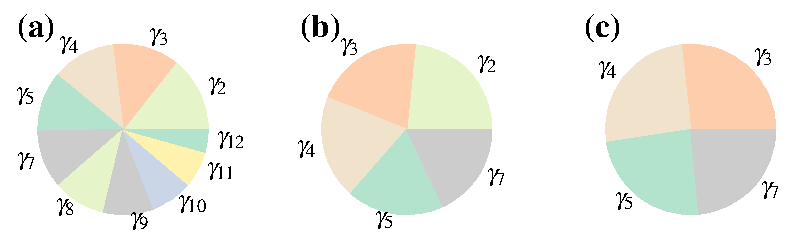
\includegraphics{theoretical_study/figures/knapsack_roulette.pdf}
    \end{center}
    \caption[Roulette wheels for selection]{
        Roulette wheels showing selection probability $s_i$ for corresponding candidates $\gamma_i$. 
        Colours here only distinguish candidates, they do not encode any information. 
        \textbf{b}, The set of potential parents is truncated to include only the strongest five candidates. 
        \textbf{a}, All valid candidates are assigned selection probability based on their value in \cref{table:knapsack_candidates}. 
        \textbf{c}, After one parent ($\gamma_2$) has been chosen, it is removed from the roulette wheel and the remaining
         candidates' probabilities are renormalised for the selection of the second parent. 
    }
    \label{fig:knapsack_roulette}
\end{figure}

A key subroutine of every \gls{ga} is the mechanism through which it nominates candidates from generation $\mu$ 
as parents to offsping candidates in $\mu+1$ \cite{luke11}. 
All mechanisms have in common that they act on a set of candidates from the previous generation, 
    where each candidate, $\gamma_j$, has been evaluated and has fitness value, $g_j$. 
Among the viable schemes for selecting individual parents from the set of candidates, $\mu$  are
\begin{easylist}[itemize]
    & Rank selection: candidates are selected with probabilty proportional to their ranking relative to 
        the fitness of contemporary candidates in the same generation;
    & Tournament selection: a subset of $k$ candidates are chosen at random from $\mu$, 
        of which the candidate with the highest fitness is taken as the parent;
    & Stochastic universal sampling: candidates are sampled proportional to their fitness, 
        but the sampling algorithm is biased to ensure high-fitness candidates are chosen at least once 
        within the generation. 
\end{easylist}

We will only detail the mechanism used in later applications within this thesis: 
    fitness proportional selection, known as \emph{roulette selection} \cite{luke11}. 
This is a straightforward strategy where we directly map candidates' fitness, $g_i$ to a selection probability, $s_i$,
    simply by normalising $\{g_i\}$, 
    allowing us to visualise a roulette wheel of uneven wedges, each of which correspond to a candidate. 
Then we need only conceptually spin the roulette wheel to select the first parent, $\gamma_{p_1}$. 
We then remove $\gamma_{p_1}$ from the set of potential parents, renormalise the remaining $\{s_i\}$, 
    and spin the wheel again to choose the second parent, $\gamma_{p_2}$. 
The roulette selection is shown in \cref{fig:knapsack_roulette}.
\par 

Practically, we repeat the process outlined until the next generation is filled, 
    usually we have $|\mu| = N_m$, and desire that every generation should contain the same 
    $N_m$ candidates, so we repeat the roulette selection $\nicefrac{N_m}{2}$ times per generation, 
    since every pair of parents yield two offspring.
It is important that meaningful differences in fitness are reflected by the selection probability, 
    which is difficult to ensure for large $N_m$, e.g. with ten models, the strongest candidate is only 
    a marginally more probable parent than the worst -- this effect is amplified for larger $N_m$. 
We therefore wish to reduce the set of potential parents to ensure high quality offspring:
    we truncate $\mu$ and retain only the highest-fitness $\frac{N_m}{2}$ models as selectable parents. 
\par 

\subsection{Reproduction}
\label{sec:reproduction}
\begin{figure}
    \begin{center}
        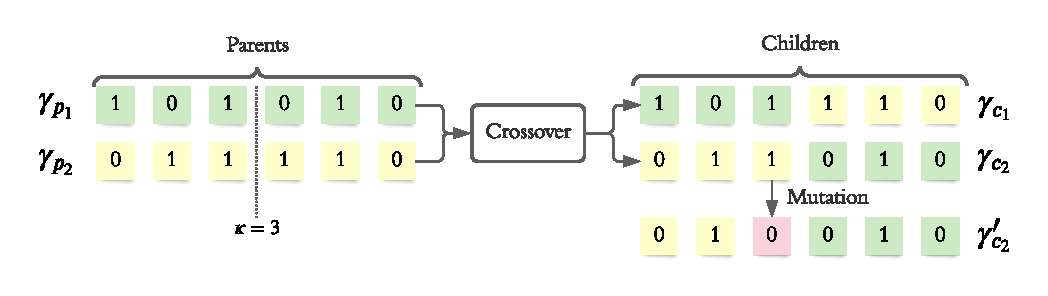
\includegraphics{theoretical_study/figures/chromosomes.pdf}
    \end{center}
    \caption[Crossover and mutation of chromosomes.]{
        Crossover and mutation of chromosomes.
        Two parents, $\left\{\gamma_{p_1}, \gamma_{p_2}\right\}$, are nominated from the process in \cref{fig:knapsack_roulette}. 
        They are then crossed-over via a one-point crossover with crossing point $\kappa=3$, 
        resulting in children candidates $\left\{\gamma_{c_1}, \gamma_{c_2}\right\}$. 
        One child chromosome is mutated to yield a new candidate, $\gamma_{c_2}^{\prime}$. 
        The candidates added to the next generation are then $\{ \gamma_{c_1}, \gamma_{c_2}^{\prime} \}$.
    }
    \label{fig:gen_alg_reproduction}
\end{figure}

When a pair of parents have been nominated by the selection mechanism above, 
    it remains to use those parents to \emph{reproduce}, 
    i.e. to produce offspring which should inherit and improve upon the properties of their parents. 
Here we use a \emph{one point crossover}, whereby the two parent chromosomes are mixed together 
    to form two offspring, about a single point, $\kappa$: 
    for candidates of $n$ genes, 
    the first $\kappa$ genes of $\gamma_{p_1}$ are conjoined with the latter $n - \kappa$ genes of $\gamma_{p_2}$. 
Often $\kappa$ is restricted to the midpoint of the chromosomes, although in general we need not impose this: 
    we will instead consider $\kappa \in \left( \frac{n}{4}, \frac{3n}{4} \right)$, 
    e.g. with $n=12$, $\kappa \in (3, 9)$. 
The one-point crossover is shown for $n=6$ with $\kappa=3$ in \cref{fig:gen_alg_reproduction}, 
    recalling the chromosome structure from \cref{sec:knapsack}.
\par 
By allowing $\kappa$ other than the midpoint, we drastically increase the number of combinations of parents available for reproduction. 
Finally, then, parent selection is done by constructing a database of pairs of potentital parents with all available crossover points, 
    with selection probability given by the product of their individual fitnesses. 
This is conceptually equivalent to selection via roulette wheel as above. 
Recalling the fitnesses (values) of \cref{table:knapsack_candidates}, we generate the parent selection database:

\begin{table}[H]
    \begin{center}
        \begin{tabular}{cccc}
            Parent 1 & Parent 2 & $\kappa$ & $s_{ij}$ \\
            \hline 
            $\gamma_2$ & $\gamma_3$ & 2 & $11,187 \ (=113 \times 99 )$ \\
            $\gamma_2$ & $\gamma_3$ & 3 & $11,187$ \\
            $\gamma_2$ & $\gamma_3$ & 4 & $11,187$ \\

            $\gamma_2$ & $\gamma_4$ & 2 & $10,735 \ (=113 \times 95)$ \\
            $\gamma_2$ & $\gamma_4$ & 3 & $10,735$ \\
            $\gamma_2$ & $\gamma_4$ & 4 & $10,735$ \\

             & & \vdots & \\

            $\gamma_5$ & $\gamma_7$ & 2 & $7,743 \ (=89 \times 87)$ \\
            $\gamma_5$ & $\gamma_7$ & 3 & $7,743$ \\
            $\gamma_5$ & $\gamma_7$ & 4 & $7,743$ \\

        \end{tabular}
    \end{center}
    \caption[Genetic algorithm parent selection database]{
        Example of parent selection database. 
        Pairs of parents are selected together, with the (unnormalised) selection probability, $s_{ij}$, 
        given by the product of the individual candidates' fitnesses. 
        Pairs of parents are repeated in the database for differing $\kappa$, 
            and all $\kappa$ are equally likely. 
    }
    \label{table:selection_database}
\end{table}
    

The \gls{ga} maintains diversity in the subspace of $\population$ it studies, 
    by \emph{mutating} some of the newly proposed offspring candidates. 
Again, there are a multitude of approaches for this step \cite{schmitt2001theory}, 
    but for brevity we only describe those used in this thesis.
For each proposed child candidate, $\gamma_{c}$, we probabilistically mutate each gene with some mutation rate $r_m$:
    if a mutation occurs, the child is replaced by $\gamma_c^{\prime}$. 
That is, $\gamma_c^{\prime}$  is added to the next generation, and $\gamma_c$ is discarded. 
$r_m$ is a \emph{hyperparameter} of the \gls{ga}:
    the performance of the algorithm can be optimised by finding the best $r_m$ 
    for a given problem. 

\subsection{Candidate evaluation}
\label{sec:candidate_evaluation}
Within every generation of the \gls{ga}, each candidate must be evaluated, 
    so that the relative strength of candidates can be exploited in constructing 
    candidates for the next generation.
In the example of the knapsack problem used above, candidates were evaluated by the value of their contents, 
    but also by whether they would fit in the knapsack. 
Idenitfiyng the appropriate method by which to evaluate candidates is arguably the most important aspect of designing a \gls{ga}:
    while the choice of hyperperameters ($N_g, N_m, r_m$) dictate the efficacy of the search, 
    the lack of an effective metric by which to distinguish candidates would render the procedure pointless.
Considerations are hence usually built into the \glsentryfull{of};
    \glspl{ga} implementations later in this thesis therefore demand we design \glspl{of} 
    with respect to the individual application. 
\par 




